\documentclass[a4paper]{article}

%use the english line for english reports
%usepackage[english]{babel}
\usepackage[portuguese]{babel}
\usepackage[utf8]{inputenc}
\usepackage{indentfirst}
\usepackage{graphicx}
\usepackage{verbatim}
\usepackage[margin=0.8in]{geometry}
\usepackage{amsmath}
\usepackage{listings}
\lstset{language=Prolog}  

\begin{document}

\setlength{\textwidth}{16cm}
\setlength{\textheight}{22cm}

\title{\Huge\textbf{Sixteen Stone}\linebreak\linebreak\linebreak
\Large\textbf{Relatório Intercalar}\linebreak\linebreak
\linebreak\linebreak

\includegraphics[scale=0.1]{images/feup-logo.png}\linebreak\linebreak
\linebreak\linebreak
\Large{Mestrado Integrado em Engenharia Informática e Computação} \linebreak\linebreak
\Large{Programação em Lógica}\linebreak
}

\author{\textbf{Grupo Sixteen\_Stone\_3:}\\
Diogo Filipe Costa - ei11014 \\
Maria Teresa Chaves - up201306842 \\
\linebreak\linebreak \\
 \\ Faculdade de Engenharia da Universidade do Porto \\ Rua Roberto Frias, s\/n, 4200-465 Porto, Portugal \linebreak\linebreak\linebreak
\linebreak\linebreak\vspace{1cm}}

\maketitle
\thispagestyle{empty}

%----------------------------------------------------------------------------------------------------------------------------------------------------------------------
%----------------------------------------------------------------------------------------------------------------------------------------------------------------------

\newpage

%Todas as figuras devem ser referidas no texto. %\ref{fig:codigoFigura}
%
%%Exemplo de código para inserção de figuras
%%\begin{figure}[h!]
%%\begin{center}
%%escolher entre uma das seguintes três linhas:
%%\includegraphics[height=20cm,width=15cm]{path relativo da imagem}
%%\includegraphics[scale=0.5]{path relativo da imagem}
%%\includegraphics{path relativo da imagem}
%%\caption{legenda da figura}
%%\label{fig:codigoFigura}
%%\end{center}
%%\end{figure}
%
%
%\textit{Para escrever em itálico}
%\textbf{Para escrever em negrito}
%Para escrever em letra normal
%``Para escrever texto entre aspas''
%
%Para fazer parágrafo, deixar uma linha em branco.
%
%Como fazer bullet points:
%\begin{itemize}
	%\item Item1
	%\item Item2
%\end{itemize}
%
%Como enumerar itens:
%\begin{enumerate}
	%\item Item 1
	%\item Item 2
%\end{enumerate}
%
%\begin{quote}``Isto é uma citação''\end{quote}


%----------------------------------------------------------------------------------------------------------------------------------------------------------------------

\tableofcontents
\listoffigures

\newpage

%----------------------------------------------------------------------------------------------------------------------------------------------------------------------

\section{O Jogo Sixteen Stone}

Sixteen Stone é o nome de um jogo de tabuleiro abstrato \footnote{Jogo abstrato - jogo de estratégia que tenta minimizar a sorte e não possui tema.}\footnote{Informação obtida em https://pt.wikipedia.org/wiki/Jogo\_de\_estrat\%C3\%A9gia\_abstrato} de forma quadrada, jogado normalmente num tabuleiro de 5x5, para dois jogadores. Inicialmente, cada jogador tem 8 pedras vermelhas ou azuis, colocando-as de forma alternada em qualquer uma das células livres, sendo que o jogador vermelho é o primeiro a jogar. Assim que todas as pedras estejam no tabuleiro, o jogo começa. O jogo termina quando o jogador vencedor consegue reduzir para um o número de pedras em jogo do adversário.

\subsection{Tabuleiro de jogo}

Esta secção tem como objetivo introduzir o tabuleiro de jogo e os elementos que dele fazem parte.

\begin{figure}[!htb]
	\centering
	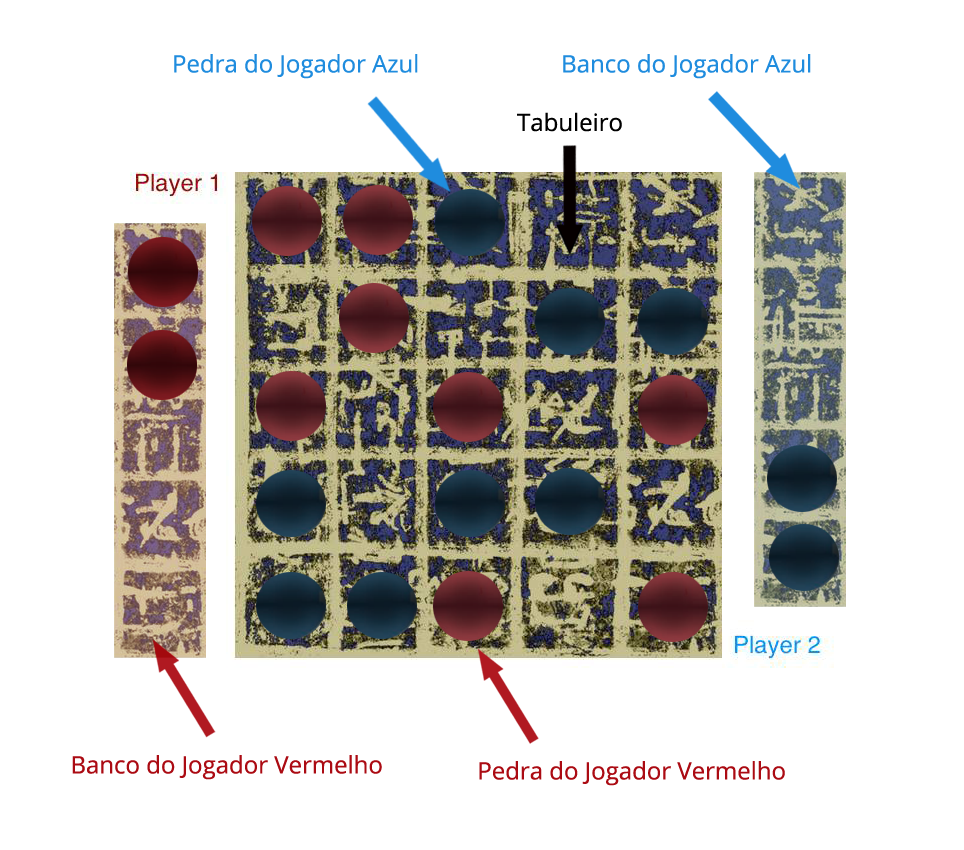
\includegraphics[scale=0.3]{images/board_explained.png} 
	\caption{Explicação do tabuleiro.}
\end{figure}

Elementos do tabuleiro:

\begin{itemize}
	\item \textbf{Pedras} - cada jogador possui um certo número de pedras, sendo que o jogador 1 possui as pedras vermelhas e o 2 as pedras azuis.
	\item \textbf{Banco} - cada jogador possui um banco onde estão guardadas as pedras que não estão em jogo.
	\item \textbf{Tabuleiro} -  onde os jogadores colocam as suas pedras de jogo e podem efetuar vários movimentos.
\end{itemize}

\newpage

\subsection{Regras}

No início do jogo distribui-se 8 pedras (vermelhas ou azuis) para cada jogador. De forma alternada os jogadores devem colocá-las em qualquer uma das células livres, começando as pedras vermelhas.

\begin{figure}[!htb]
	\centering
	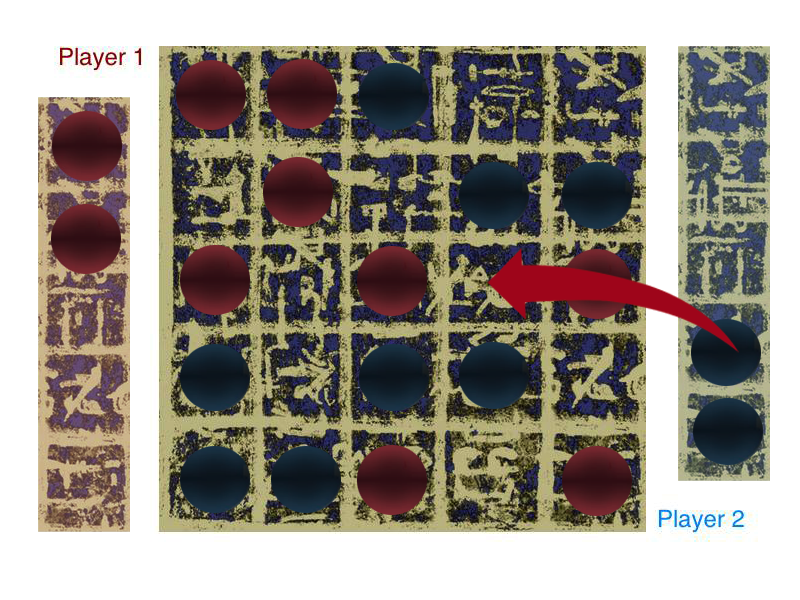
\includegraphics[scale=0.3]{images/board_prep.png}
	\caption{Preparação do tabuleiro.}
\end{figure}

Quando as pedras estiverem todas colocadas no tabuleiro, o jogador vermelho começa a jogar e alterna de turno com o jogador adversário.

\subsubsection{Jogadas possíveis}

Um jogador pode no seu respetivo turno realizar cada uma das seguintes jogadas: \textit{Push}, \textit{Move} e \textit{Sacrifice}.
No primeiro turno de cada jogador, deve ser feito um \textit{Push} ou um \textit{Move}, mas nunca ambos.

\begin{figure}[!htb]
	\centering
	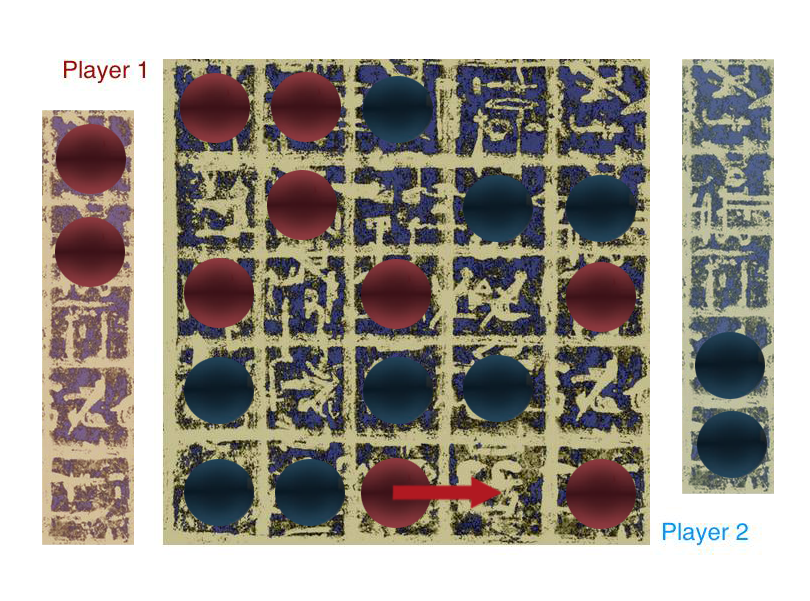
\includegraphics[scale=0.3]{images/first_move.png}
	\caption{Jogador vermelho realiza um \textit{Move} no seu primeiro turno.}
\end{figure}

\newpage

\subsubsection{\textit{Push}}

Para realizar um  \textit{Push} é necessário que o jogador tenha mais pedras nessa linha que o adversário. Assim, se após um  \textit{Push}, a pedra do adversário é "empurrada" para fora do tabuleiro, então vai para o "banco" do respetivo jogador. As pedras que são "empurradas" apenas se movem uma célula na direção do \textit{Push}, que pode ser realizado em qualquer direção.

\begin{figure}[!htb]
	\centering
	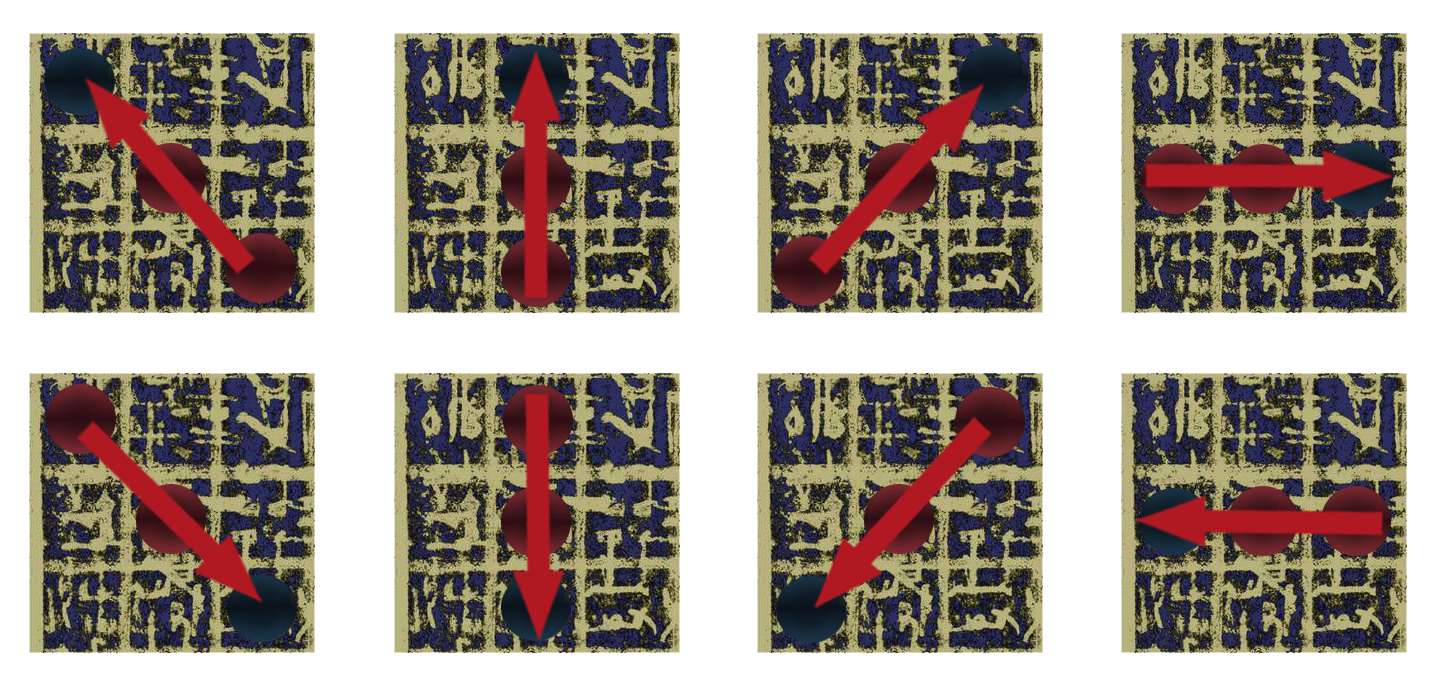
\includegraphics[scale=0.3]{images/push_dirs.png} 
	\caption{Direções possíveis de um \textit{Push} e situações em que a pedra do adversário é "empurrada" para fora do tabuleiro.}
\end{figure}

\begin{figure}[!htb]
	\centering
	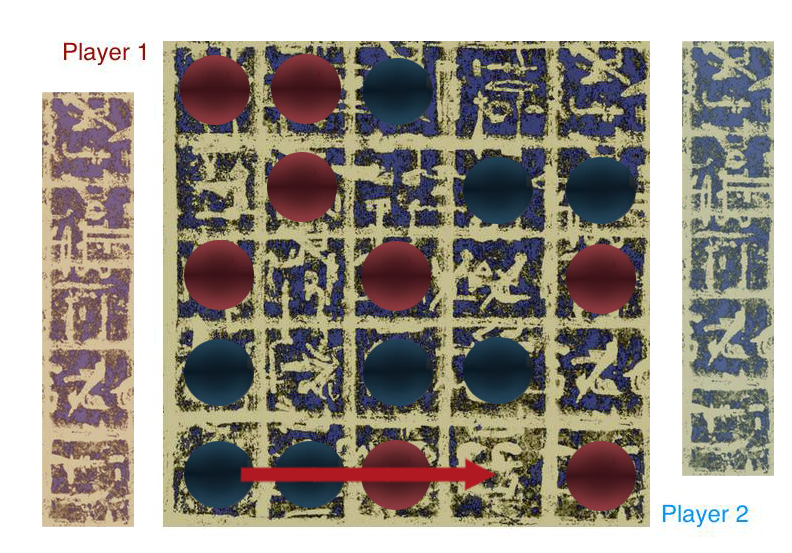
\includegraphics[scale=0.3]{images/push_not_poll.png} 
	\caption{\textit{Push} sem que a pedra adversária seja "empurrada" para fora do tabuleiro.}
\end{figure}

O número de pedras máximo (PE) que um jogador pode "empurrar" é igual a:

\begin{equation}
	PE = P - 1 \text{\hspace{7mm}(sendo P o número das suas pedras nessa linha)}
\end{equation}

\newpage

Isto é, por exemplo, caso numa linha o jogador azul tenha três pedras, então pode realizar um  \textit{Push} a uma pedra ou a duas do adversário. Mas caso tenha duas apenas pode realizar um  \textit{Push} a uma pedra vermelha.

\begin{figure}[!htb]
	\centering
	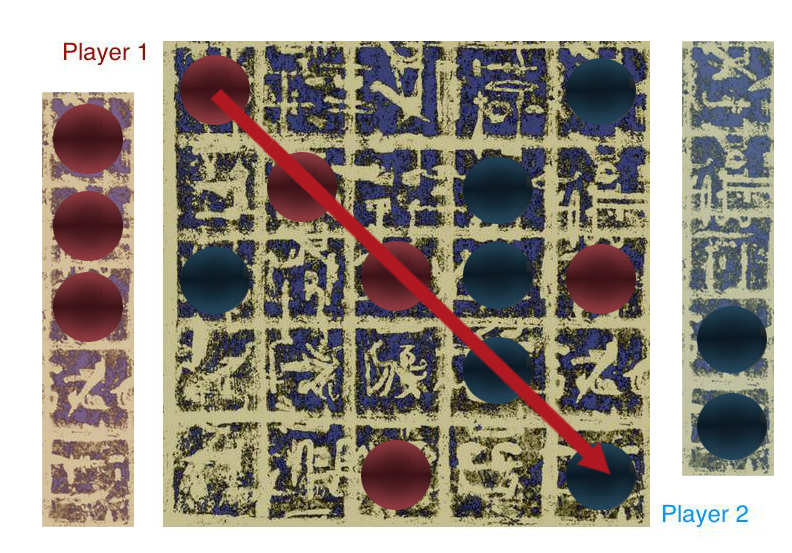
\includegraphics[scale=0.3]{images/push_3_stones.png}
	\caption{Push com três pedras.}
\end{figure}

Além das regras referidas anteriormente, um jogador não pode realizar um  \textit{Push} nas suas próprias pedras.
Por fim, para realizar um \textit{Push} é necessário que exista uma pedra para ser "empurrada". Por exemplo, caso numa coluna o jogador vermelho tenha duas pedras, mas nessa coluna o jogador vermelho não tem pedras, então realizar um  \textit{Push} é uma jogada inválida.

\begin{figure}[!htb]
	\centering
	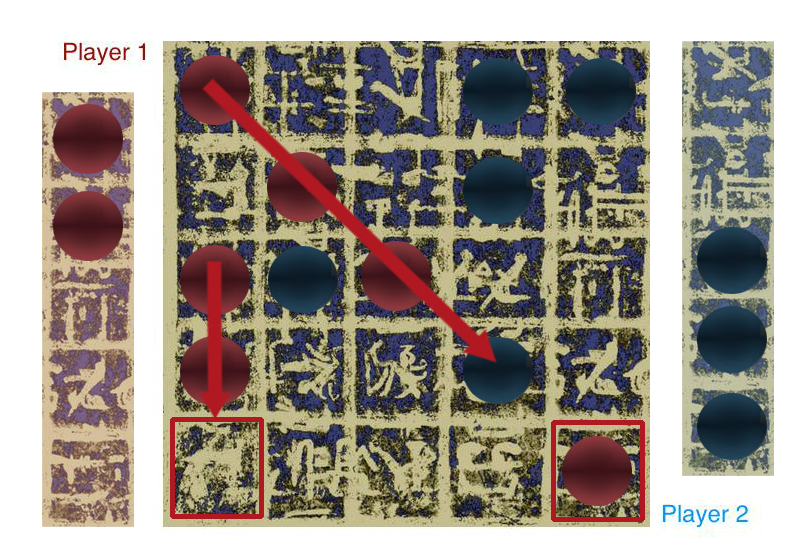
\includegraphics[scale=0.3]{images/invalid_push.png} 
	\caption{Push inválido: nas suas próprias pedras (a); numa célula vazia (b).}
\end{figure}

\newpage

\subsubsection{\textit{Move}}

É possível realizar um  \textit{Move} para uma célula vazia em qualquer direção. Se o jogador tentar realizar um \textit{Move} para uma célula ocupada, então é considerado uma jogada inválida.

\begin{figure}[!htb]
	\centering
	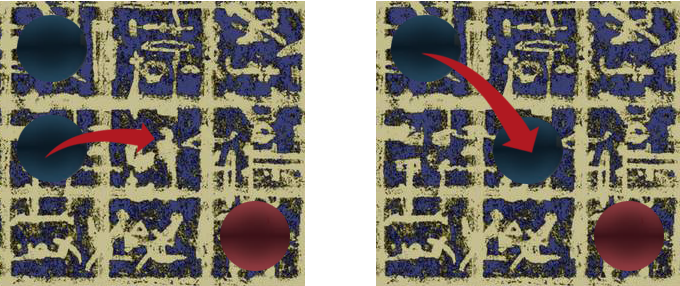
\includegraphics[scale=0.2]{images/valid_invalid_move.png} 
	\caption{\textit{Move} válido (a) e um \textit{Move} inválido (b).}
\end{figure}

Após um \textit{Move} se alguma das pedras adversárias ficar cercada\footnote{Uma pedra fica cercada quando existem pelo menos em duas direções opostas pedras adversárias.}, então esta é capturada e substituída por uma pedra do "banco" do jogador que a capturou.

\begin{figure}[!htb]
	\centering
	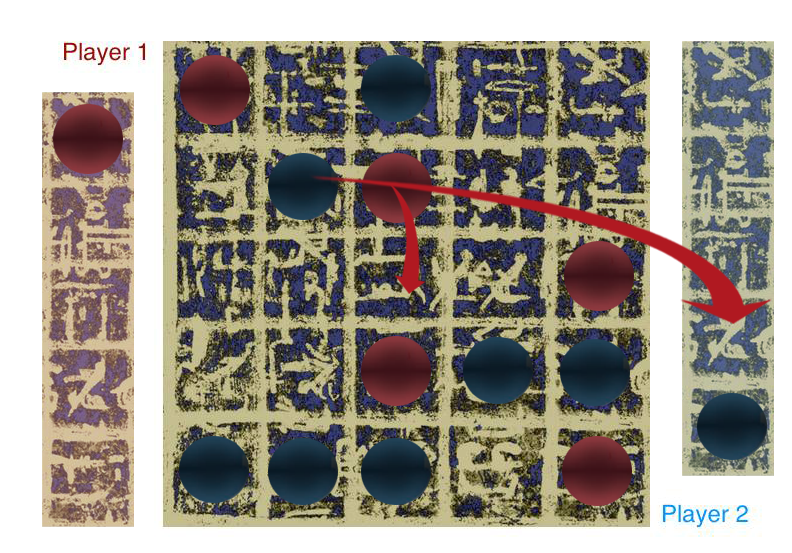
\includegraphics[scale=0.3]{images/move_cap.png} 
	\caption{Pedra azul capturada após um \textit{Move} de uma pedra vermelha.}
\end{figure}

Se um jogador realizar um \textit{Move} e a sua pedra ficar voluntariamente cercada, esta não é capturada.

\begin{figure}[!htb]
	\centering
	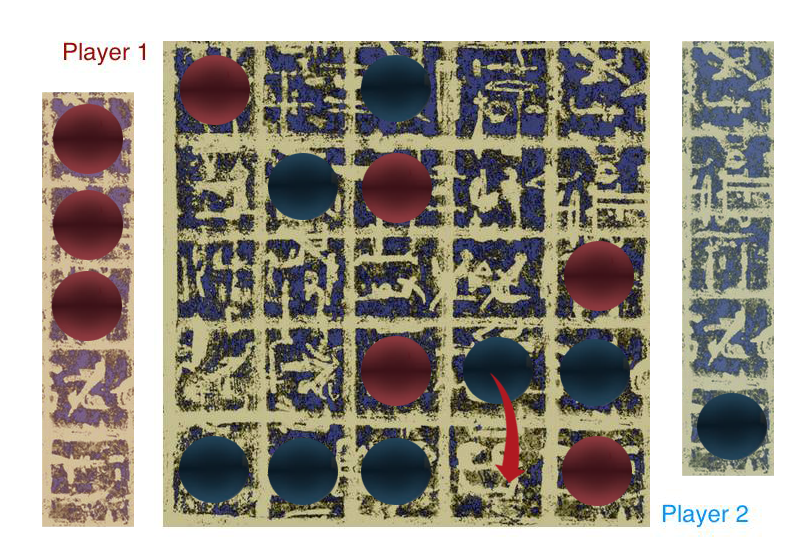
\includegraphics[scale=0.3]{images/move_no_cap.png} 
	\caption{Pedra que após um \textit{Move} não é capturada.}
\end{figure}

\subsubsection{\textit{Sacrifice}}

Um jogador pode sacrificar uma pedra do seu "banco", permanentemente, para poder realizar um \textit{Push} ou um \textit{Move} adicional.

\begin{figure}[!htb]
	\centering
	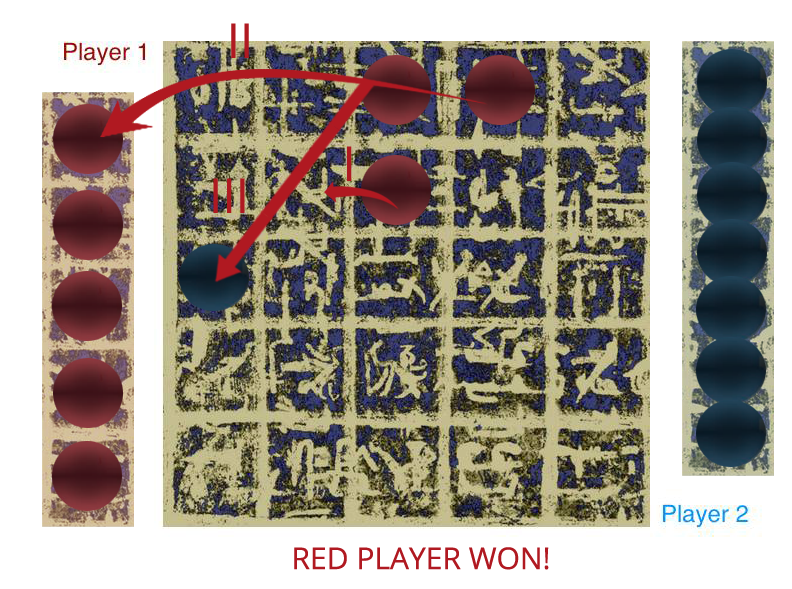
\includegraphics[scale=0.3]{images/sacrifice.png}
	\caption{Jogador azul realiza um \textit{Move} (I), um \textit{Sacrifice} (II) e depois um \textit{Push} (III) e ganha o jogo.}
\end{figure}

%----------------------------------------------------------------------------------------------------------------------------------------------------------------------
\newpage

\section{Representação do Estado do Jogo}

O tabuleiro é representado por uma lista de listas  $L = \{L_1, L_2, ... , L_n\} , n > 0  \wedge n$ é múltiplo de $5$, em que $n$ é a dimensão do tabuleiro. \par
Com o predicado \texttt{make\_board} é possível criar um tabuleiro (\textit{Board}) com um tamanho \textit{Size}. Para isso o \texttt{make\_board} utiliza o predicado \texttt{make\_line} para criar uma linha e depois usa o \texttt{make\_board} recursivamente. De forma a tornar mais clara a visualização do tabuleiro de jogo, após criá-lo com o \texttt{make\_board} utiliza-se o predicado \texttt{print\_board} que o imprime no ecrã.

\begin{figure}[!htb]
	\centering
	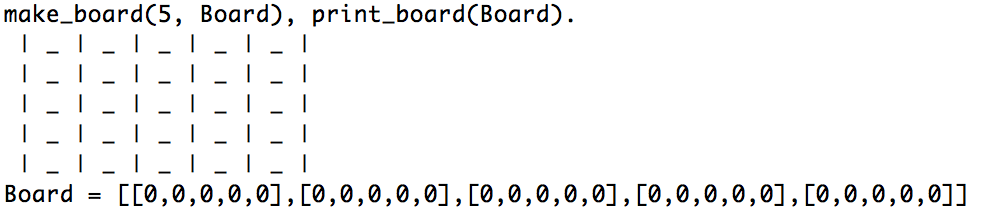
\includegraphics[scale=0.6]{images/make_board.png}
	\caption{Estado inicial do jogo.}
\end{figure}

A figura acima demonstra o estado do tabuleiro na sua fase inicial, sem nenhuma célula preenchida. De uma forma mais visual, segue-se abaixo uma figura demonstrativa do tabuleiro.

\begin{figure}[!htb]
	\centering
	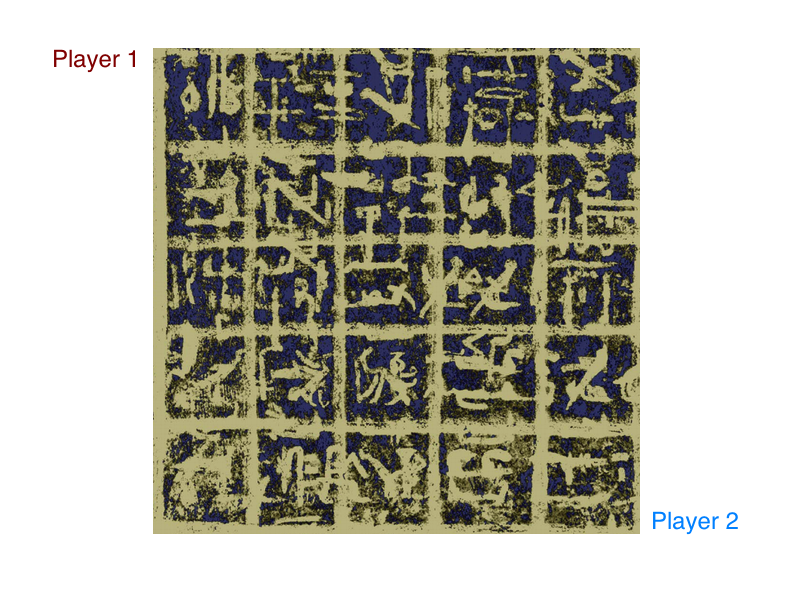
\includegraphics[scale=0.3]{images/board.png}
	\caption{Tabuleiro de jogo.}
\end{figure}

O jogador pode realizar cada uma das três jogadas possíveis: \textit{Push}, \textit{Move} e \textit{Sacrifice}. Para o \textit{Push} é usado o predicado \texttt{push(Stone\_src, Stone\_dst, Dir, Board)}, onde \texttt{Stone\_src} e \texttt{Stone\_dst} são as coordenadas x-y (separadas por um traço) das pedras inicial e destino, \texttt{Dir} é a direção do \textit{Push} e pode ter os valores: 0 (cima), 1 (direita), 2 (baixo) ou 3 (esquerda) e \texttt{Board} é o tabuleiro que é retornado após o \textit{Push}.

\begin{figure}[!htb]
	\centering
	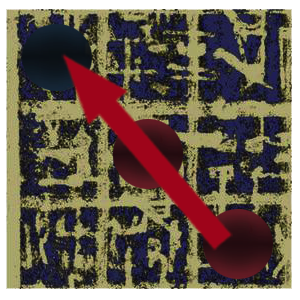
\includegraphics[scale=0.2]{images/push.png}
	\caption{Exemplo de um \textit{Push}.}
\end{figure}

\newpage

Para o \textit{Move} é usado o predicado \texttt{move(Stone\_src, Cell\_dst, Board)}, onde \texttt{Stone\_src} é a pedra que se pretende mover, \texttt{Cell\_dst} é a célula de destino e o \texttt{Board} é o tabuleiro que é retornado.

\begin{figure}[!htb]
	\centering
	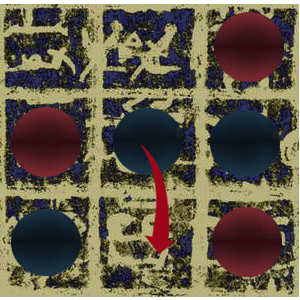
\includegraphics[scale=0.3]{images/move.png}
	\caption{Exemplo de um \textit{Move}.}
\end{figure}

Para o \textit{Sacrifice} é usado o predicado \texttt{sacrifice(Stone, Board)}, onde \texttt{Stone} é a pedra que se pretende sacrificar e o \texttt{Board} é o tabuleiro que é retornado.

\begin{figure}[!htb]
	\centering
	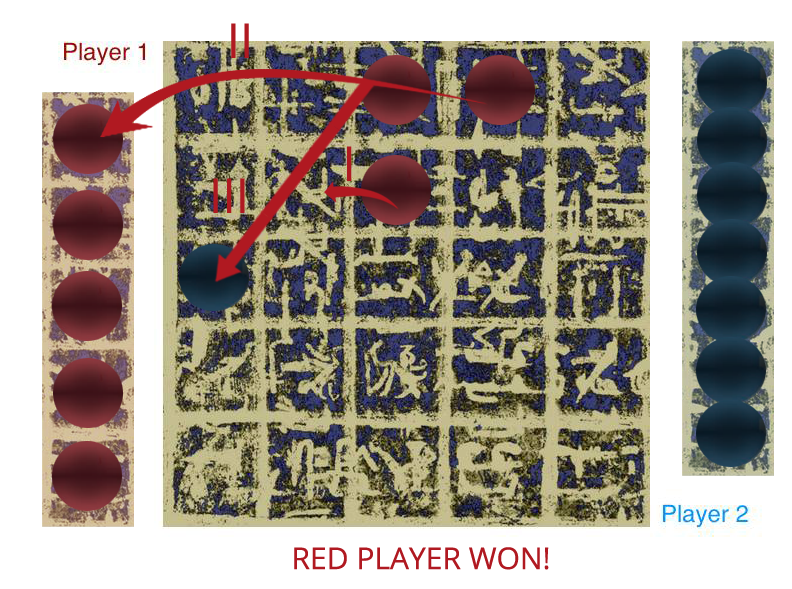
\includegraphics[scale=0.3]{images/sacrifice.png}
	\caption{Exemplo de um \textit{Sacrifice} (II).}
\end{figure}

Existe ainda um predicado \texttt{moveToPool(Stone, Player, Pool)} que move uma uma pedra (\texttt{Stone}) para o "banco" de um dado jogador (\texttt{Player}) retorna o "banco" do jogador (\texttt{Pool}) após a pedra ter sido movida.

\begin{figure}[!htb]
	\centering
	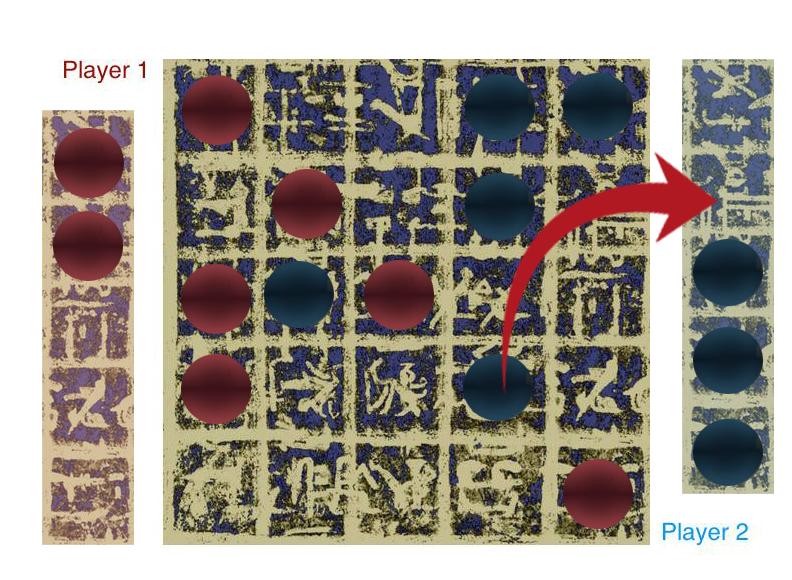
\includegraphics[scale=0.2]{images/pool.png}
	\caption{Exemplo de uma pedra a ser colocada no "banco" de um jogador.}
\end{figure}

\newpage

%----------------------------------------------------------------------------------------------------------------------------------------------------------------------
\section{Visualização do Tabuleiro}

A cor das pedras dos jogadores são representadas pelos carateres \texttt{x} para as pedras azuis e \texttt{o} para as pedras vermelhas, sendo que o carater \texttt{\_} é usado para representar casas vazias.

Os predicados utilizados para construir e visualizar o tabuleiro são:

\begin{itemize}
	\item \texttt{make\_line/2} - Gera uma linha do tabuleiro
	\item \texttt{make\_board/2} - Gera um tabuleiro de jogo com o tamanho especificado
	\item \texttt{print\_line/1} - Predicado para imprimir uma linha do tabuleiro
	\item \texttt{print\_board/1} - Predicado que imprime o tabuleiro, passado sob a forma de uma lista de listas
	\item \texttt{draw\_board/2} - Predicado que chama os predicados anteriores para gerar um tabuleiro com um tamanho especificado e imprime-o no ecrã
\end{itemize}

\begin{figure}[!htb]
	\centering
	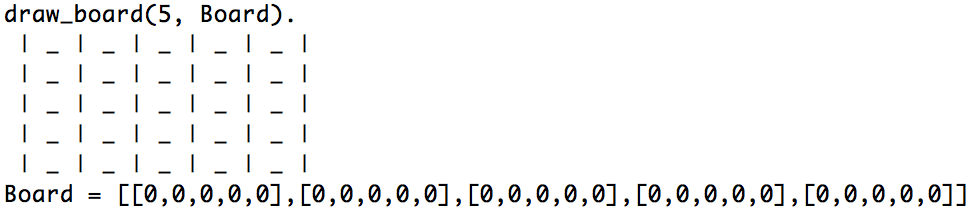
\includegraphics[scale=0.6]{images/draw_board.png}
	\caption{Exemplo de chamada do predicado \texttt{draw\_board} para um tamanho de 5x5}
\end{figure}

Numa fase já intermédia do jogo, o tabuleiro poderá atingir um ponto com o seguinte o formato:

\begin{figure}[!htb]
	\centering
	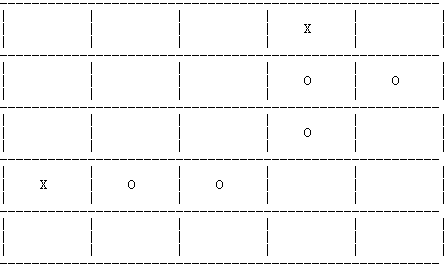
\includegraphics[scale=0.5]{images/board_prolog.png}
	\caption{Exemplo de fase intermédia do jogo.}
\end{figure}

De uma forma mais visual, segue-se abaixo uma figura ilustrativa da fase respetiva do tabuleiro.

\begin{figure}[!htb]
	\centering
	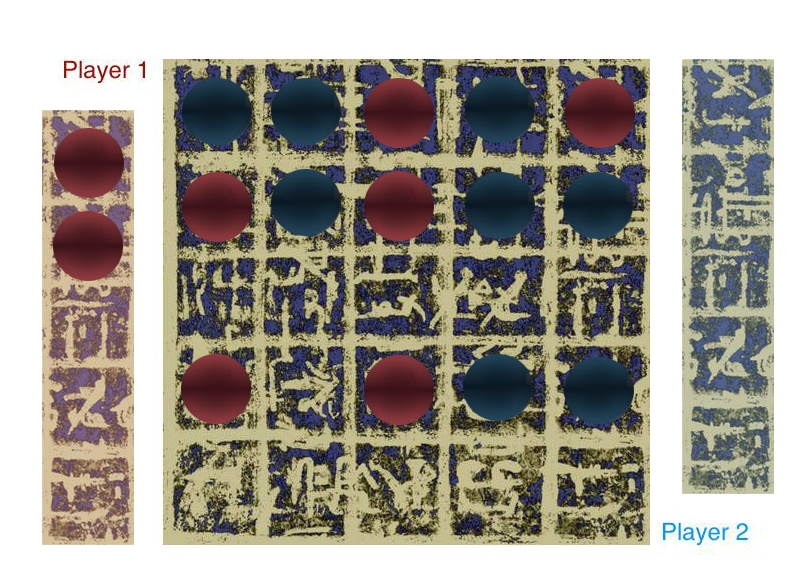
\includegraphics[scale=0.6]{images/board_inter.png}
	\caption{Forma mais visual de uma fase intermédia do jogo.}
\end{figure}

\newpage

%----------------------------------------------------------------------------------------------------------------------------------------------------------------------
\section{Movimentos}

Elencar os movimentos (tipos de jogadas) possíveis e definir os cabeçalhos dos predicados que serão utilizados (ainda não precisam de estar implementados).

\newpage

\section*{Bibliografia}

"Jogo de estratégia abstrato", https://pt.wikipedia.org/wiki/Jogo\_de\_estrat\%C3\%A9gia\_abstrato (acedido em 7 de Outubro de 2015) \newline

"Sixteen Stone", http://www.boardgamegeek.com/boardgame/173193/sixteen-stone (acedido em 7 de Outubro de 2015) \newline

"Sixteen Stone - rules v.1.0", http://www.boardgamegeek.com/filepage/117073/sixteen-stone-rules-v10 (acedido em 7 de Outubro de 2015) \newline

\end{document}
